\chapter{Administrarea spațiului de stocare}
\label{chapter:storage}

În cadrul unui sistem de calcul, unitatea de procesare este elementul central,
cel care realizează operațiile necesare, respectiv cerute, de către utilizator.
Pentru a putea realiza aceste operații, unitatea de procesare are nevoie de un
mecanism prin care să fie aduse datele la aceasta cât mai rapid și de un
mecanism prin care să furnizăm rezultatele înapoi utilizatorului. Cel mai
apropiat mecanism de intrare/ieșire a datelor necesare/rezultate este memoria
(RAM și cache-urile aferente). Principalul dezavantaj al memoriei o reprezintă
volatilitatea: la pierderea alimentării cu energie electrică, datele stocate în
memorie se pierd. Pentru a preîntâmpina această problemă, a fost introdus un nou
nivel de intrare/ieșire a datelor în care capacitatea de înmagazinare a datelor
este net superioară, iar la întreruperea alimentării cu energie electrică,
datele se păstrează. Acest nou nivel de intrare/ieșire poartă denumirea, în
general, de dispozitiv de stocare. Dispozitivele de stocare au ca principal
dezavantaj viteza de operare, de aceea nu le folosim direct în relația cu
unitatea de procesare (datele trec prin memorie înainte de a ajunge la
procesor). Un alt dezavantaj al dispozitivelor de stocare îl reprezintă modul
modul de organizare a datelor pe acesta: capacitatea este net superioară
comparativ cu a unei memorii (gigabytes vs. terabytes/petabytes) iar o adresare
liniară, ca în cazul memoriei, nu ar fi posibilă. În cadrul acestui capitol vom
studia tehnici de organizare a datelor pe dispozitivele de stocare (vezi
\labelindexref{Figura}{fig:storage-mem-struct}.

\begin{figure}[htbp]
	\centering
	\def\svgwidth{\columnwidth}
	\includesvg{chapters/10-storage/img/mem-struct.svg}
	\caption{Ierarhia de memorie în cadrul unui sistem de calcul}
	\label{fig:storage-mem-struct}
\end{figure}

Așadar, stocarea este și ea un element central în operațiile cu sistemul de
calcul. Orice informație procesată ar trebui stocată persistent pe un
dispozitiv. Dispozitivele de stocare, după cum a fost prezentat și în
\labelindexref{Capitolul}{chapter:hardware}. Componente hardware, sunt alcătuite
din două componente: controller și discuri. Controller-ul este asemenea unei
unități de procesare din cadrul unui sistem de calcul, dar specializat în
controlul și managementul unităților de stocare (discurilor). Controller-ele au
rolul de a centraliza logica de acces la unitățile de stocare și de a nu duplica
logica în cadrul fiecărui disc. De asemenea, deoarece discurile sunt cu câteva
ordine de mărime mai lente comparativ cu unitatea de procesare, controller-ul
acționează ca un element intermediar de control: procesorul dă comanda
controller-ului, acesta execută toate operațiile cerute și când sunt finalizate,
anunță unitatea principală de execuție (procesorul). Astfel procesorul nu
așteaptă după unitățile de stocare, ci execută alte operații relevante în tot
acest timp. În \labelindexref{Figura}{fig:storage-concurent} este reprezentat un
exemplu de transfer de date de la o locație de pe Internet în timp de
utilizatorul folosește aplicația \textit{Calculator}. Discurile sunt cele ce
stochează efectiv informația. Luăm ca exemplu aplicațiile Google Drive și
Dropbox: acestea oferă servicii de stocare a informațiilor pentru utilizatori.
Pentru a implementa facilitățile de stocare și partajare a datelor, aceste
aplicații folosesc sisteme de stocare. În secțiunea următoare vom descrie și vom
realiza o clasificare a discurilor.

\begin{figure}[!htbp]
	\centering
	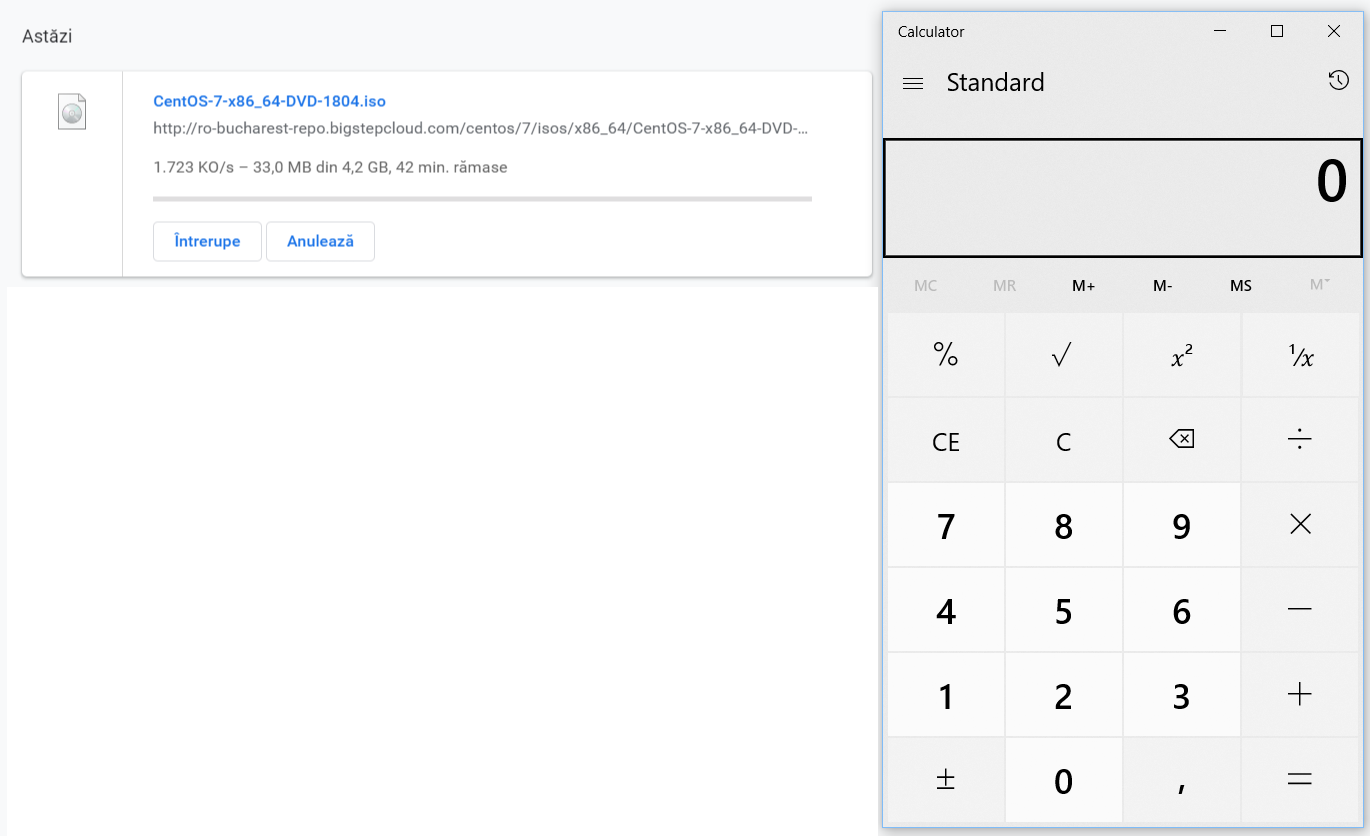
\includegraphics[width=15cm]{chapters/10-storage/img/concurent-img.png}
	\caption{Executarea concomitentă a transferului de date și a unei aplicații}
	\label{fig:storage-concurent}
\end{figure}

\section{Tipuri de discuri}
\label{sec:storage-tipuri}

Subsistemul de stocare din cadrul unui sistem de calcul este format dintr-un
controller care furnizează partea de logică a transferului de date și de unul
sau mai multe discuri care stochează efectiv informația. Dispozitivele de
stocare au următoarele atribute principale:

\begin{itemize}
	\item spațiul disponibil - câtă informație se poate stoca pe disc
		(măsurat de obicei în gigabytes - GB sau terabytes
		\abbrev{TB}{terrabytes} - TB)
	\item viteza de acces - cât de repede se pot transfera datele de pe disc
		în memoria RAM (măsurat de obice în megabytes pe secundă - MB/s)
	\item mod de poziționare - intern (în interiorul unității) sau extern
		(în exteriorul unității)
	\item mod de conectare - există două tipuri de conectare pentru
		discurile interne (SATA vs. SAS) și un tip de conectare în
		general pentru cele externe (USB)
	\item fiabilitate - câte ore de funcționare sau câte citiri/scrieri
		suportă de-a lungul vieții de funcționare. Aceste numere variază
		mult în funcție de tipul unității de stocare (HDD vs. SSD) și de
		gama pentru care a fost proiectat (folosirea în desktop-uri vs.
		servere)
\end{itemize}

În zilele noastre există două tipuri de discuri pe sistemele de calcul:

\begin{itemize}
	\item Hard Disk Drive (HDD)
	\item Solid State Drive (SSD \abbrev{SSD}{Solid State Drive})
\end{itemize}

\subsection{Hard Disk Drive}
\label{sec:storage-tipuri-hdd}

HDD-ul prin construcție dispune de părți mobile în interiorul acestuia: un braț
de citire/scriere si unul sau mai multe platane pe care se stochează datele
(vezi \labelindexref{Figura}{fig:storage-hdd}). Astfel HDD-ul este predispus defectării atunci când acesta
funcționează și este supus unor anumite șocuri mecanice. De asemenea șocurile
mecanice sunt problematice și atunci când HDD-ul nu funcționează (platanele nu
se rotesc, iar capul de citire/scriere nu se mișcă). Modelul constructiv al
HDD-ului de asemenea nu permite viteze de funcționare ridicate comparativ cu
memoria RAM. Parametri prin care se măsoară performanța unui HDD sunt: numărul
de rotații pe minut al platanelor și viteza interfeței de conectare la
controller în gigabiți pe secundă. În zilele noastre, există două tipuri de
interfețe de conectare:

\begin{itemize}
	\item SATA - Serial ATA \abbrev{SATA}{Serial Advanced Technology
		Attachment} (Serial Advanced Technology Attachment)
	\item SAS - Serial Attached SCSI \abbrev{SAS}{Serial attached SCSI} (sau
		Serial Attached Small Computer System Interface)
\end{itemize}

\begin{figure}[!htbp]
	\centering
	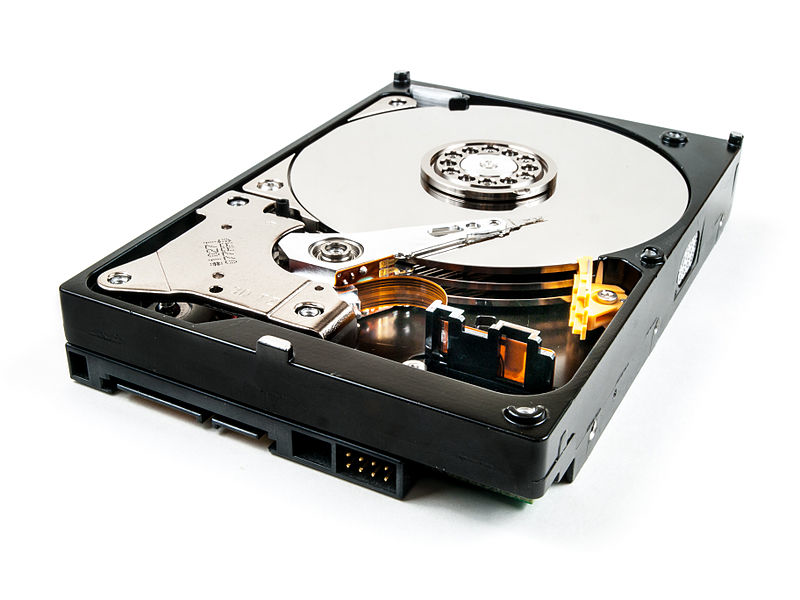
\includegraphics[width=8cm]{chapters/10-storage/img/hdd-img.png}
	\caption{HDD\protect\footnotemark}
	\label{fig:storage-hdd}
\end{figure}

\footnotetext{\url{https://commons.wikimedia.org/wiki/File:Hard_Drive_(11644419853).jpg}
\textbf{CC BY 2.0}}

În funcție de aceste interfețe se clasifică și discurile. Ambele interfețe se
interconectează cu controller-ul în general la o viteză de 6Gbps. Discurile cu
interfețe de tip SATA au viteza de rotație mai redusă decât SAS (5400rpm/7200rpm
vs 10000rpm/15000rpm), iar durata de viață, din construcție, este mult mai mică
decât a SAS-urilor. De aceea discurile SATA sunt cu mult mai ieftine decât
discurile SAS de aceeași capacitate (în cele mai multe cazuri pentru aceeași
capacitate prețul se dublează). Un alt deziderat al discurilor SATA este acela
că se concentrează pe capacitatea de stocare, iar discurile SAS se concentrează
pe viteza de funcționare. Din cauza prețului foarte ridicat al discurilor SAS,
acestea se folosesc în servere și sisteme de tip enterprise, iar discurile SATA
se folosesc în calculatoarele personale.

În \labelindexref{Figura}{fig:storage-sas-sata} sunt reprezentate cele 2 tipuri
de interfețe: în stânga sunt interfețe de tip SATA, iar în dreapta de tip SAS.

\begin{figure}[!htbp]
	\centering
	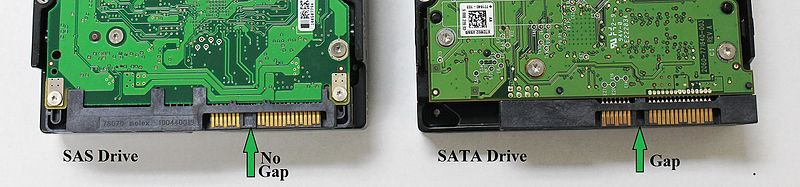
\includegraphics[width=8cm]{chapters/10-storage/img/sas-sata-img.png}
	\caption{SATA vs SAS\protect\footnotemark}
	\label{fig:storage-sas-sata}
\end{figure}

\footnotetext{\url{https://commons.wikimedia.org/wiki/File:SASvsSATA_Connector.JPG}
\textbf{CC BY SA 3.0}}

\begin{figure}[!htbp]
	\centering
	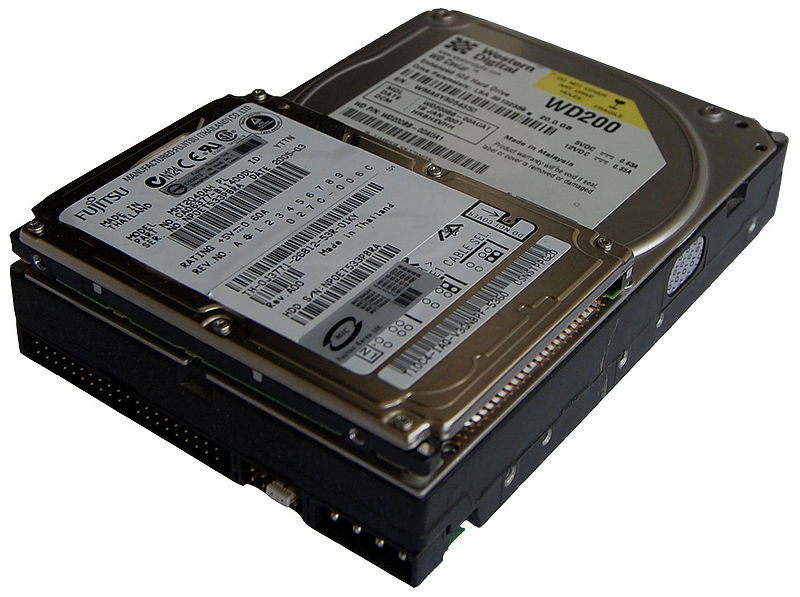
\includegraphics[width=8cm]{chapters/10-storage/img/size-comp-img.png}
	\caption{2.5" vs 3.5"\protect\footnotemark}
	\label{fig:storage-size-comp}
\end{figure}

\footnotetext{\url{https://commons.wikimedia.org/wiki/File:Comparison_of_3.5_and_2.5_inch_hard_drives.jpg}
\textbf{CC BY SA 3.0}}

O altă clasificare a discurilor este legată de mărimea fizică a acestora:

\begin{itemize}
	\item 2.5 inch (discurile de deasupra din Fig. X)
	\item 3.5 inch (discurile de dedesubt din Fig. X)
\end{itemize}


Discurile de 2.5 inch se folosesc de obicei în sisteme enterprise, unde se
dorește economisirea spațiului sau acomodarea a cât mai multe HDD-uri într-o
unitate (1U).

\subsection{SSD}
\label{sec:storage-tipuri-ssd}

SSD-ul a venit ca un răspuns la neajunsurile HDD-ului, încercând să
îmbunătățească sensibilitatea la șocuri precum și viteza de funcționare a
acestuia. SSD-ul nu are părți mobile în interiorul acestuia și funcționează pe
principiul stick-urilor USB: pentru a stoca informația se folosesc chip-uri
construite din semiconductoare și nu discuri/platane magnetice care prezintă o
mișcare pentru a putea citi/scrie datele.

Discurile de tip SSD pot fi conectate atât printr-o interfață SATA ce oferă
viteze de până la 6Gbps cât și printr-o interfață SAS ce oferă viteze de până la
12Gbps în acest moment. Forma constructivă a unui SSD este atât de 2.5 inch cât
și de 3.5 inch, similar HDD-urilor.

Costul SSD-urilor comparativ cu cel al HDD-urilor, în special la capacități de
peste 1TB este semnificativ mai mare (de aproximativ 5 ori). De aceea în
sistemele din ziua de astăzi există un disc principal SSD unde se stochează
sistemul de operare și aplicațiile care au nevoie de acces rapid la acesta și un
HDD de mare capacitate pentru stocarea datelor de termen lung și care nu
necesită viteză ridicată.

Un aspect de luat în considerare atunci când se achiziționeză un disc de tip SSD
este durata de viață. Spre deosebire de un HDD, SSD-ul are un număr limitat de
scrieri specificat de producător, după care se spune că s-a finalizat durata de
viață a acestuia. Din acest motiv, sistemele de operare și sistemul de fișiere
trebuie să întreprinde operații specifice, optimizate pentru SSD-uri, pentru a
le prelungi durata de viață (de exemplu defragmentarea generează foarte multe
scrieri, scurtând durata de viață a discului, iar aceasta nu este utilă pentru
un SSD - viteza de citire a oricăror date aleator de pe disc este aceeași în
cazul SSD-urilor). Pentru a afla durata de viață a unui disc SSD există tool-uri
speciale cum ar fi SSD Life (https://ssd-life.com).


Pentru a prelungi durata de viață a unui disc, ca utilizator, trebuie să aveți
în vedere următoarele facilități:

\begin{itemize}
	\item Defragmentarea (procesul prin care se rearanjează datele pe disc
		pentru un acces mai eficient) - este recomandată dezactivarea
		defragmentării pentru discurile SSD (dupa cum am specificat mai
		sus)
	\item Swapping - atunci când un sistem rămâne fără memorie RAM, acesta
		va folosi pe post de memorie discul. Este recomandat să
		dezactivați swapping-ul pe discurile SSD dacă doriți prelungirea
		duratei de viață (mai ales dacă swapping-ul apare des)
	\item Hibernate - atunci când trecem calculatorul în starea Hibernate
		acesta scrie întregul conținut al memoriei pe disc (ceea ce va
		genera foarte multe scrieri). Este recomandat să nu treceți
		sistemul în Hibernate dacă doriți prelungirea duratei de viață
		(sau să configurați un disc alternativ pentru Hibernate).
\end{itemize}

Alte recomandări pentru creșterea duratei de viață a discului SSD specifice
sistemului de operare folosit, le puteți găsi la o simplă căutare pe Google
%(ex.:
%https://www.makeuseof.com/tag/3-top-tips-maintain-performance-extend-life-ssd-si/).

\section{Partiționarea dispozitivelor de stocare}
\label{sec:storage-part}

În secțiunile anterioare au fost prezentate caracteristicile discurilor, atât
SSD cât și HDD. O caracteristică principală a acestora este capacitatea mare de
stocare (mult mai care ca a memoriei RAM). Așadar o adresare liniară nu este
suficientă pentru a gestiona spațiul de stocare oferit de un disc. Mai mult, un
alt motiv este constituit de faptul că administrarea spațiului de stocare este
făcută de către utilizator în schimb administrarea zonei de memorie RAM este
făcută de către sistemul de operare. Astfel administrarea spațiului de stocare
trebuie să fie simplă și facilă.

Spațiul de stocare oferit de un dispozitiv trebuie administrat în mod corect
pentru a asigura o stocare eficientă (performanță ridicată) și coerentă (să nu
corupem date). Există 2 nivele de administrare: partiționare și sistemele de
fișiere. Aceste nivele sunt interdependente și se aplică iterativ.

Partiționarea împarte spațiul disponibil în diverse zone contigue, fiecare zonă
având un specific definit de la creare (partiție de boot, partiție pentru
utilizatori, partiție pentru sistemul de de operare). Există două tipuri de
partiționări în sistemele din ziua de astăzi, așa cum am prezentat în
\labelindexref{Capitolul}{chapter:boot}:

\begin{itemize}
	\item Master Boot Record (referit ca MBR) - acesta a fost introdus în
		1983 și poartă această denumire deoarece stochează la începutul
		discului un sector specific procesului de bootare.
	\item GUID Partition Table (referit ca GPT) - este o metodă mai nouă de
		partiționare ce va înlocui treptat MBR-ul din cauza limitărilor
		acestuia.
\end{itemize}

MBR-ul, după cum se menționează anterior, are alocat exact la începutul unui
disc un sector special de boot care reține schema de partiționare precum și o
versiune minimală a boot loader-ului care va încărca sistemul de operare (vezi
8. Pornirea sistemului). Schema de partiționare MBR este formată din maxim 4
partiții, denumite primare. Pentru a acoperi aceste neajunsuri, au fost
introduse partițiile logice: una din partițiile primare va fi alocată pe întreg
discul rămas liber și va fi marcată ca partiție extinsă. În cadrul partiției
extinse se pot crea oricâte partiții logice se dorește. Acest lucru îngreunează
schema de partiționare, iar unele sisteme de operare nu pot porni folosind
aceste partiții. Nu se recomandă folosirea acestor partiții, ca partiții de
bootare. Întreaga schemă de partiționare a MBR este descrisă și în
\labelindexref{Figura}{fig:storage-mbr-struct}.

\begin{figure}[htbp]
	\centering
	\def\svgwidth{\columnwidth}
	\includesvg{chapters/10-storage/img/mbr-struct.svg}
	\caption{Schema de partiționare a MBR}
	\label{fig:storage-mbr-struct}
\end{figure}

MBR-ul a început să fie înlocuit de către GPT din cauza limitărilor acestuia,
cum ar fi:

\begin{itemize}
	\item Dimensiunea maximă a unei partiții este de 2TB
	\item Necesitatea unei partiții extinse pentru a crea mai mult de patru partiții
\end{itemize}

Pentru a rezolva neajunsurile MBR-ului, a fost creată schema de partiționare
GPT. Numele GUID Partition Table (GPT) vine de la faptul că fiecare partiție a
discului are asociat un număr unic de identificare (guid), generat aleator și
care garantează că fiecare partiție de pe glob va avea propriul identificator
unic.

GPT-ul este asociat în general cu standardul UEFI care dorește înlocuirea
BIOS-ul în sistemele de calcul. BIOS-ul și UEFI-ul sunt programe low-level care
se execută la pornirea sistemelor de calcul pentru a realiza testarea și
inițializarea componentelor. UEFI-ul este un nou standard, menit să înlocuiască
BIOS-ul pentru a acoperi neajunsurile acestuia (mai multe detalii sunt
prezentate în \labelindexref{Capitolul}{chapter:boot}. Pornirea sistemului).

În \labelindexref{Figura}{fig:storage-gpt-struct} este reprezentată schema de
partiționare a GPT-ului. Se observă asemănarea cu partiționarea de tip MBR: la
începutul discului există MBR-ul. După MBR se află header-ul GPT ce descrie
partițiile (maxim 128). MBR-ul și header-ul sunt duplicate și la finalul
discului: în caz de corupere a primelor sectoare să nu pierdem detaliile despre
schema de partiționare. În cazul GPT nu mai avem limitarea la 2TB a unei
partiții și nici limitarea la 4 partiții primare (din cauza numărului ridicat
disponibil de partiții nu mai există noțiunea de partiții logice).

\begin{figure}[htbp]
	\centering
	\def\svgwidth{\columnwidth}
	\includesvg{chapters/10-storage/img/gpt-struct.svg}
	\caption{Schema de partiționare a GPT}
	\label{fig:storage-gpt-struct}
\end{figure}

Pentru a utiliza spațiul de stocare eficient, există recomandări din partea
vendorilor sistemelor de operare. Bunele practici în partiționarea unui disc
includ:

\begin{itemize}
	\item Crearea unei partiții de boot (specific Linux /boot - conține
		nucleul sistemului de operare și boot-lodear-ul)
	\item Crearea unei partiții de swap (specific Linux - spațiu utilizat de
		sistemul de operare atunci când rămâne fără memorie; în cazul
		Windows swap-ul este alocat din partiția sistemului de operare)
	\item Crearea unei partiții pentru sistemul de operare (pentru Linux
		este /, denumită și root, iar pentru Windows de obicei este
		discul C:).
	\item Crearea unei partiții pentru utilizatorii sistemului - atunci când
		reinstalăm sistemul de operare, să putem păstra ușor datele
		utilizatorilor (pentru Linux este /home, iar pentru Windows de
		obicei literele de la D: în sus)
	\item Crearea unei partiții pentru sistemele cu suport EFI/UEFI
		(specific Linux în /boot/efi și conține fișierele necesare să
		fie executate la încărcarea sistemului de operare de către
		subsistemul UEFI)
\end{itemize}

Utilitare ce pot fi folosite pentru administrarea partițiilor sunt:

\begin{itemize}
	\item Pentru Linux: fdisk (doar MBR); parted/gparted (suport extins
		pentru MBR/GPT și operații avansate). O dată creată o partiție,
		aceasta poate fi văzută în calea /dev și poartă numele discului
		partiționat (ex. sda) urmat de o cifră care reprezintă numărul
		partiției (ex. sda5)
	\item Pentru Windows: Disk Management. O data creată o partiție, aceasta
		poate fi văzută în utilitarul menționat.
\end{itemize}

\subsection{Sisteme de fișiere}
\label{sec:storage-fs}

Pentru a putea organiza datele pe o partiție într-un mod facil și ușor de
înțeles pentru utilizatorul final al sistemului de calcul, pe aceasta în general
se instalează un sistem de fișiere. Procesul de instalare/alocare a unui sistem
de fișiere pe o partiție se numește formatare. O partiție fără un sistem de
fișiere nu poate fi utilizată/explorată de către utilizatorul final. De exemplu,
pe Windows, un disc USB neformatat nu va putea fi accesat cu dublu-click și va
apărea un mesaj către utilizator dacă acceptă formatarea lui (vezi
\labelindexref{Figura}{fig:storage-format-disk})

\begin{figure}[!htbp]
	\centering
	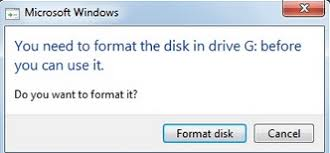
\includegraphics[width=8cm]{chapters/10-storage/img/format-disk-img.png}
	\caption{Fereastră privind formatarea unui disc pe Windows}
	\label{fig:storage-format-disk}
\end{figure}

Sistemul de fișiere oferă următoarele obiecte vizibile utilizatorului final:

\begin{itemize}
	\item Fișierul - entitatea care conține date utile în diverse formate
	\item Directorul - entitatea care organizează fișierele într-un formă
		arborescentă ușor de folosit de către utilizator.
\end{itemize}

Mai multe detalii legate de fișiere și directoare (modul în care se crează, se
șterg, permisiuni de acces) puteți citi în
\labelindexref{Capitolul}{chapter:file-system}. Utilizarea sistemului de
fișiere.

În general sistemele de fișiere sunt specifice sistemelor de operare. Astfel avem următoarea clasificare:

\begin{itemize}
	\item Linux: cel mai folosit este sistemul de fișiere ext4, iar mai nou
		acesta ajunge să fie înlocuit cu xfs
	\item Windows: principalul sistem de fișiere este NTFS
\end{itemize}

Pe Linux pentru a formata (instala) un sistem de fișiere pe o partiție se
folosește comanda \cmd{mkfs}. urmată de sufixul sistemului de operare dorit și
partiția dorită (ex. \textit{mkfs.ext4 /dev/sda2}). ATENȚIE: procesul de
formatare a unui sistem de fișiere distruge datele prezente pe acea partiție. O
greșeala frecventă este aplicarea procesului de formatare pe între discul (ex.
\cmd{mkfs.ext4 /dev/sda}). Acest lucru va șterge \textbf{toate} partițiile de pe
acel disc. Un exemplu complet de folosire a utilitarelor de formatare și
partiționare îl puteți găsi la finalul capitolului, la studii de caz.

\begin{figure}[!htbp]
	\centering
	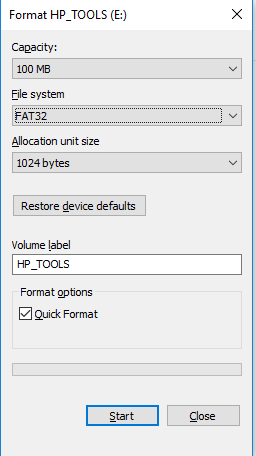
\includegraphics[width=8cm]{chapters/10-storage/img/format-part-img.png}
	\caption{Formatarea unei partiții pe Windows}
	\label{fig:storage-format-part}
\end{figure}

Pe Windows pentru a formata (instala) un sistem de fișiere pe o partiție, se
face click dreapta pe litera aferentă partiției și există opțiunea Format: de
aici se poate selecta tipul sistemului de fișiere și diverse caracteristici de
formatare (vezi \labelindexref{Figura}{fig:storage-format-part}).

Pentru a putea folosi un sistem de fișiere, acesta trebuie făcut disponibil
utilizatorului. Procesul prin care acest este disponibil pentru citire/scriere
se numește montare.

Pe sistemele bazate pe Linux, montarea se realizează cu comanda mount urmată de
partiția care se dorește a fi montată și locația unde să fie montată în sistemul
de fișiere:

\begin{screen}
[root@monitor ~]# mount /dev/sdb1 /mnt/
[root@monitor ~]# mount | grep sdb1
/dev/sdb1 on /mnt type ext4 (rw)
\end{screen}

Un lucru specific sistemelor de operare bazate pe Linux este alocarea unui ID
la formatarea unei partiții. Astfel la montare se poate specifica ID-ul
partiției și nu calea către device. Acest lucru este utilizat pentru a rezolva
conflictele generate de schimbarea ordinii discurilor fizice. De exemplu, în
cazul prezentat mai sus, dacă mai inserăm un disc fizic în sistem, acesta poate
fi detectat înainte celui prezent și i se va aloca litera b, deci va fi sdb, iar
cel curent va deveni sdc. Astfel comanda de mai sus devine invalidă și
inconsistentă deoarece va monta un cu totul alt disc. Pentru a afla ID-ul alocat
unei partiții noi formatate se folosește comanda blkid:

\begin{screen}
[root@monitor ~]# blkid /dev/sdb1
/dev/sdb1: UUID="ae064abe-b2fb-402b-8ba1-4ab1293bb584" TYPE="ext4"
\end{screen}

Acum putem monta partiția folosind acest ID notat cu UUID (Unique Univerally
Identifier):

\begin{screen}
mount -U ae064abe-b2fb-402b-8ba1-4ab1293bb584 /mnt/
\end{screen}


Pe sisteme Windows montarea se realizează în general automat de către sistemul
de operare. Dacă se doresc operații avansate, acestea pot fi făcute tot din
\textit{Disk Management} (Start -> Run -> diskmgmt.msc; vezi Fig. X):

\begin{figure}[!htbp]
	\centering
	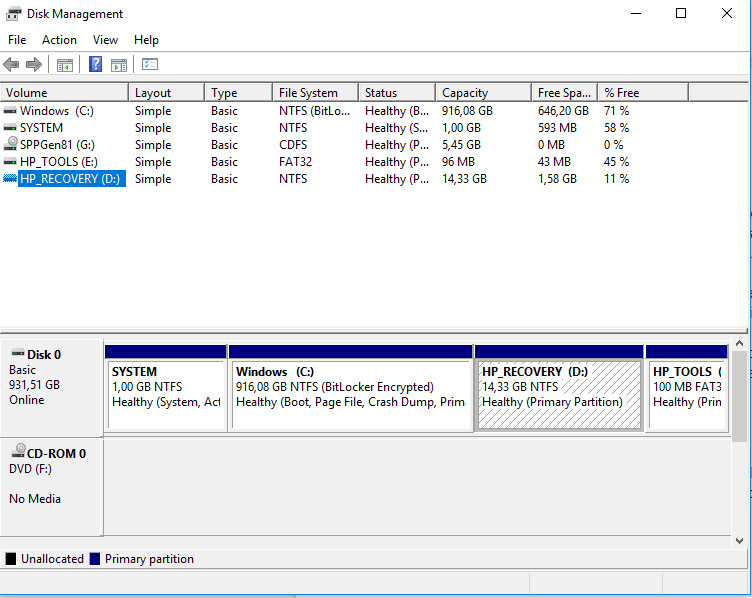
\includegraphics[width=8cm]{chapters/10-storage/img/admin-img.png}
	\caption{Administrarea spațiului de stocare pe Windows}
	\label{fig:storage-admin}
\end{figure}

Anterior, s-a menționat faptul că sistemele de fișiere sunt specifice sistemului
de operare. La nevoie, aceste sisteme de fișiere se pot monta pe alt sistem de
operare decât cele pentru care au fost proiectate. Acest lucru nu este
întotdeauna recomandat întrucât există penalități de performanță și risc de
corupere a datelor.

Sistemele de fișiere au mecanisme interne de recuperare a datelor corupte.
Principalul mecanism prin care se realizează acest lucru este jurnalizarea (file
system journal). Fiecare sistem de fișiere scrie fiecare operație adusă
sistemului de fișiere într-un jurnal. Atunci când sunt probleme la montarea unui
sistem de fișiere, acesta folosește jurnalul pentru a încerca să repare
inconsistențele. De multe ori nu se poate monta sistemul de fișiere fără o
verificare completă a integrității sistemului de fișiere. Acest lucru se
realizează de obicei automat la pornirea sistemului de operare, atât pe Linux
cât și Windows. Este important de menționat faptul că nu toate sistemele de
fișiere oferă suport de jurnalizare. În ziua de astăzi sisteme de fișiere care
nu oferă acest suport este datorat faptului că sunt simple prin construcția lor
și se adresează dispozitivelor specializate (e.g. camere video) și cu puține
resurse care nu au implementat un mecanism de verificare a integrității (e.g.
sistemul de fișiere FAT).

Pe Linux, dacă este necesară verificarea integrității sistemului de fișiere
manual, se poate folosi utilitarul \cmd{fsck}:

\begin{screen}
[root@monitor ~]# fsck /dev/sdb1
fsck from util-linux-ng 2.17.2
e2fsck 1.43-WIP (20-Jun-2013)
/dev/sdb1 is mounted.
e2fsck: Cannot continue, aborting.
\end{screen}

Se observă că nu se poate verifica sistemul de fișiere când acesta este deja
montat. Vom demonta sistemul de fișiere iar apoi vom verifica integritatea:

\begin{screen}
[root@monitor ~]# umount /mnt/
[root@monitor ~]# fsck /dev/sdb1
fsck from util-linux-ng 2.17.2
e2fsck 1.43-WIP (20-Jun-2013)
/dev/sdb1: clean, 11/13272 files, 6616/52916 blocks
\end{screen}

Ca și schemele de partiționare, sistemele de fișiere au și ele anumite limitări
legate de:

\begin{itemize}
	\item Numărul maxim de fișiere (ex. Pentru ext4 - 4 miliarde)
	\item Dimensiunea partiției (ex. pentru ext4 - 1024PB)
	\item Dimensiunea maximă a fișierului (ex. Pentru ext4 - 16TB)
	\item Atribute extinse de funcționalitate și securitate
\end{itemize}

Limitările menționate mai sus variază de la un sistem de operare la altul, iar
acestea pot fi aflate citind documentația respectivului sistem de fișiere.

Până în acest punct am discutat despre disc și partiție. Discul este partea
fizică a sistemului de calcul disponibilă spre a fi folosită de către sistemul
de operare. Pentru o folosire eficientă, acesta este partiționat (partiție).
Deseori, prin diverse tehnici (RAID hardware sau software - vezi secțiunea
următoare), mai multe discuri sunt puse la comun și văzute ca unul singur.
Rezultatul poartă numele de \textit{volum}. Un alt termen folosit în
administrarea spațiului de stocare este \textit{drive}. Acesta are două
semnificații: referă tot un disc fizic sau referă o partiție pe sisteme Windows.

\section{Anexă: Investigarea spatiului de stocare}
\label{sec:storage-investigare}

Pe un sistem Linux, pentru a vizualiza toate discurile din sistem, precum și
unde sunt montate, putem folosi comanda \cmd{lsblk}:

\begin{screen}
[root@monitor ~]# lsblk
NAME   MAJ:MIN RM  SIZE RO TYPE MOUNTPOINT
sda      8:0    0 68.2G  0 disk
|-sda1   8:1    0  500M  0 part /boot
|-sda2   8:2    0    4G  0 part [SWAP]
|-sda3   8:3    0 63.8G  0 part /
sr0     11:0    1 1024M  0 rom
sr1     11:1    1 80.6M  0 rom
sdb      8:16   1  1.9G  0 disk
|-sdb1   8:17   1 51.7M  0 part
`-sdb2   8:18   1  1.8G  0 part
\end{screen}

Aceeași informație se poate observa folosind și comanda \cmd{df} (parametrul
\texttt{-h} este folosit pentru a afișa dimensiunea partițiilor în format ușor
de citit):

\begin{screen}
[root@monitor ~]# df -h
Filesystem      Size  Used Avail Use% Mounted on
/dev/sda3        63G   40G   21G  67% /
tmpfs           2.9G     0  2.9G   0% /dev/shm
/dev/sda1       477M   93M  359M  21% /boot
\end{screen}

Pentru a putea investiga spațiul ocupat de un anumit fișier sau director, puteți
folosi comanda \cmd{du} (parametrul \texttt{-h} este folosit pentru a afișa
dimensiunea în format ușor de citit, iar \texttt{-s} realizează suma tuturor
fișierelor din acel director):

\begin{screen}
[root@monitor ~]# du -hs /srv/
7.0G    /srv/
\end{screen}

Dacă nu folosim parametrul \texttt{-s} al comenzii \cmd{du}, atunci ni se va
afișa fiecare fișier recursiv al acelui director:

\begin{screen}
[root@monitor ~]# du -h /srv/ | less
16K     /srv/cursTemplates/etc
48K     /srv/cursTemplates/.git/hooks
20K     /srv/cursTemplates/.git/logs/refs/heads
32K     /srv/cursTemplates/.git/logs/refs/remotes/origin
36K     /srv/cursTemplates/.git/logs/refs/remotes
60K     /srv/cursTemplates/.git/logs/refs
76K     /srv/cursTemplates/.git/logs
20K     /srv/cursTemplates/.git/refs/heads
4.0K    /srv/cursTemplates/.git/refs/tags
32K     /srv/cursTemplates/.git/refs/remotes/origin
36K     /srv/cursTemplates/.git/refs/remotes
...
\end{screen}


Pentru a investiga informații despre partițiile unui disc se folosesc
utilitarele fdisk (pentru partiții MBR) sau mai nou \cmd{parted}/\cmd{gparted}
(suportă și GPT). Comanda \cmd{fdisk -l} va lista toate discurile și partițiile
unui sistem. Dacă se adaugă un parametru suplimentar (și anume calea către
discul pe care se dorește a fi inspectat), atunci doar acesta va fi afișat

\begin{screen}
[root@monitor ~]# fdisk -l /dev/sdb


Disk /dev/sdb: 1977 MB, 1977614336 bytes
61 heads, 62 sectors/track, 1021 cylinders
Units = cylinders of 3782 * 512 = 1936384 bytes
Sector size (logical/physical): 512 bytes / 512 bytes
I/O size (minimum/optimal): 512 bytes / 512 bytes
Disk identifier: 0x00000000


   Device Boot      Start         End      Blocks   Id  System
/dev/sdb1               1          28       52917   83  Linux
/dev/sdb2              29        1021     1877763   83  Linux
\end{screen}

Dacă renunțăm la parametru \texttt{-l}, vom intra în aplicația \cmd{fdisk}, de
unde vom putea printa tabela de partiții folosind comanda \texttt{p}. Pentru
alte comenzi folosiți litera \texttt{m}, indicată și în mesajul de afișare:

\begin{screen}
[root@monitor ~]# fdisk /dev/sdb


Command (m for help): p


Disk /dev/sdb: 1977 MB, 1977614336 bytes
61 heads, 62 sectors/track, 1021 cylinders
Units = cylinders of 3782 * 512 = 1936384 bytes
Sector size (logical/physical): 512 bytes / 512 bytes
I/O size (minimum/optimal): 512 bytes / 512 bytes
Disk identifier: 0x00000000


   Device Boot      Start         End      Blocks   Id  System
/dev/sdb1               1          28       52917   83  Linux
/dev/sdb2              29        1021     1877763   83  Linux


Command (m for help): m
Command action
   a   toggle a bootable flag
   b   edit bsd disklabel
   c   toggle the dos compatibility flag
   d   delete a partition
   l   list known partition types
   m   print this menu
   n   add a new partition
   o   create a new empty DOS partition table
   p   print the partition table
   q   quit without saving changes
   s   create a new empty Sun disklabel
   t   change a partition's system id
   u   change display/entry units
   v   verify the partition table
   w   write table to disk and exit
   x   extra functionality (experts only)
\end{screen}

Utilitarul \cmd{parted} se folosește în mod asemănător cu \cmd{fdisk}. Pentru a
administra un disc se rulează comanda \cmd{parted} urmată de calea către
dispozitiv:

\begin{screen}
[root@monitor ~]# parted /dev/sda
GNU Parted 2.1
Using /dev/sda
Welcome to GNU Parted! Type 'help' to view a list of commands.
(parted)
\end{screen}

Pentru a afișa tabela de partiții, folosim litera \texttt{p}:

\begin{screen}
(parted) p
Model: HUAWEI MMC Storage (scsi)
Disk /dev/sdb: 1978MB
Sector size (logical/physical): 512B/512B
Partition Table: msdos


Number  Start   End     Size    Type     File system  Flags
 1      31.7kB  54.2MB  54.2MB  primary  ext4
 2      54.2MB  1977MB  1923MB  primary
\end{screen}

Pentru mai multe opțiuni puteți folosi comanda \cmd{help}:

\begin{screen}
(parted) help
  align-check TYPE N                        check partition N for TYPE(min|opt) alignment
  check NUMBER                             do a simple check on the file system
  cp [FROM-DEVICE] FROM-NUMBER TO-NUMBER   copy file system to another partition


...
\end{screen}

\section{Anexă: Partiționare, formatare și montare pe Linux}
\label{sec:storage-partitionare}

Vom realiza pas cu pas partiționarea și formatarea unui disc pe Linux:

\begin{itemize}
	\item Folosind utilitarul \cmd{fdisk} investigăm discul \file{/dev/sdb}
		din sistem:

\begin{screen}
[root@monitor ~]# fdisk /dev/sdb


WARNING: DOS-compatible mode is deprecated. It's strongly recommended to
         switch off the mode (command 'c') and change display units to
         sectors (command 'u').


Command (m for help): p


Disk /dev/sdb: 1977 MB, 1977614336 bytes
61 heads, 62 sectors/track, 1021 cylinders
Units = cylinders of 3782 * 512 = 1936384 bytes
Sector size (logical/physical): 512 bytes / 512 bytes
I/O size (minimum/optimal): 512 bytes / 512 bytes
Disk identifier: 0x00000000


   Device Boot      Start         End      Blocks   Id  System
\end{screen}

	\item Am observat la pasul anterior că discul are 1977 MB și nu are nici
		o partiție disponibilă. Vom crea o partiție primară (se observă
		că avem opțiunea de a selecta între primar, respectiv extinsă,
		specifică partiționării MBR)

\begin{screen}
Command (m for help): n
Command action
   e   extended
   p   primary partition (1-4)
p
Partition number (1-4): 1
First cylinder (1-1021, default 1): 1
Last cylinder, +cylinders or +size{K,M,G} (1-1021, default 1021): +50M


Command (m for help): p


Disk /dev/sdb: 1977 MB, 1977614336 bytes
61 heads, 62 sectors/track, 1021 cylinders
Units = cylinders of 3782 * 512 = 1936384 bytes
Sector size (logical/physical): 512 bytes / 512 bytes
I/O size (minimum/optimal): 512 bytes / 512 bytes
Disk identifier: 0x00000000


   Device Boot      Start         End      Blocks   Id  System
/dev/sdb1               1          28       52917   83  Linux
\end{screen}

	\item Mai creăm încă o partiție cu restul de spațiu rămas:

\begin{screen}
Command (m for help): n
Command action
   e   extended
   p   primary partition (1-4)
p
Partition number (1-4): 2
First cylinder (29-1021, default 29):
Using default value 29
Last cylinder, +cylinders or +size{K,M,G} (29-1021, default 1021):
Using default value 1021


Command (m for help): p


Disk /dev/sdb: 1977 MB, 1977614336 bytes
61 heads, 62 sectors/track, 1021 cylinders
Units = cylinders of 3782 * 512 = 1936384 bytes
Sector size (logical/physical): 512 bytes / 512 bytes
I/O size (minimum/optimal): 512 bytes / 512 bytes
Disk identifier: 0x00000000


   Device Boot      Start         End      Blocks   Id  System
/dev/sdb1               1          28       52917   83  Linux
/dev/sdb2              29        1021     1877763   83  Linux
\end{screen}

	\item Vom scrie modificările pe disc:

\begin{screen}
Command (m for help): w
The partition table has been altered!


Calling ioctl() to re-read partition table.
Syncing disks.
\end{screen}

	\item Se observă că s-au creat intrări în /dev pentru fiecare partiție:

\begin{screen}
[root@monitor ~]# ls -l /dev/sdb*
brw-rw---- 1 root disk 8, 16 Aug 29 15:49 /dev/sdb
brw-rw---- 1 root disk 8, 17 Aug 29 15:49 /dev/sdb1
brw-rw---- 1 root disk 8, 18 Aug 29 15:49 /dev/sdb2
\end{screen}

	\item Pentru a putea sa o folosim, vom formata o partiție cu sistemul de
		fișiere ext4 și alta cu xfs:

\begin{screen}
root@monitor ~]# mkfs.ext4 /dev/sdb1
mke2fs 1.43-WIP (20-Jun-2013)
Filesystem label=
OS type: Linux
Block size=1024 (log=0)
Fragment size=1024 (log=0)
Stride=0 blocks, Stripe width=0 blocks
13272 inodes, 52916 blocks
2645 blocks (5.00%) reserved for the super user
First data block=1
Maximum filesystem blocks=54263808
7 block groups
8192 blocks per group, 8192 fragments per group
1896 inodes per group
Superblock backups stored on blocks:
        8193, 24577, 40961


Allocating group tables: done
Writing inode tables: done
Creating journal (4096 blocks): done
Writing superblocks and filesystem accounting information:
done
root@monitor ~]# mkfs.xfs /dev/sdb2
meta-data=/dev/sdb2              isize=256    agcount=4, agsize=32000 blks
         =                       sectsz=512   attr=2, projid32bit=1
         =                       crc=0        finobt=0, sparse=0
data     =                       bsize=4096   blocks=128000, imaxpct=25
         =                       sunit=0      swidth=0 blks
naming   =version 2              bsize=4096   ascii-ci=0 ftype=0
log      =internal log           bsize=4096   blocks=853, version=2
         =                       sectsz=512   sunit=0 blks, lazy-count=1
realtime =none                   extsz=4096   blocks=0, rtextents=0
\end{screen}

	\item Vom monta sistemul de fișiere:

\begin{screen}
[root@monitor ~]# mount /dev/sdb1 /mnt/
[root@monitor ~]# df -h | grep mnt
/dev/sdb1        47M  838K   43M   2% /mnt
\end{screen}

	\item Se observă că am alocat la partiționare 50M, dar sistemul de
		fișiere are disponibil doar 47M. Acest lucru se întâmplă din
		cauza metadatelor necesare sistemului de fișiere pentru a
		organiza datele efective.
	\item Un ultim pas pe care trebuie să îl aveți în vedere atunci când
		configurați partiționarea pe un sistem este dat de atributele
		unei partiții. Cel mai important atribut este cel care marchează
		partiția de \textit{boot}. În utilitarul \cmd{fdisk}, comanda a
		setează atributul (flag-ul) de boot pe partiția dorită (se
		observă steluța din dreptul partiției /dev/sdb2):

\begin{screen}
Command (m for help): a
Partition number (1-4): 2


Command (m for help): p


Disk /dev/sdb: 1977 MB, 1977614336 bytes
61 heads, 62 sectors/track, 1021 cylinders
Units = cylinders of 3782 * 512 = 1936384 bytes
Sector size (logical/physical): 512 bytes / 512 bytes
I/O size (minimum/optimal): 512 bytes / 512 bytes
Disk identifier: 0x00000000


   Device Boot      Start         End      Blocks   Id  System
/dev/sdb1               1          28       52917   83  Linux
/dev/sdb2   *          29        1021     1877763   83  Linux
\end{screen}

\end{itemize}

\section{Anexă: Backup periodic}
\label{sec:storage-backup}

În cadrul acestui capitol s-a discutat despre replicarea datelor. Un mod de
replicare pe lângă mecanismul RAID, este replicarea periodică a fișierelor
dintr-un sistem de operare. Acest mod de replicare este în general independent
de sistemul de fișiere.

\subsection{Backup periodic pe Linux}
\label{sec:storage-backup-linux}

În cadrul sistemelor bazate pe Linux, unul dintre cele mai folosite utilitare în
replicarea eficientă a fișierelor și directoarelor este \cmd{rsync}. Aceasta are
două caracteristici principale:

\begin{itemize}
	\item Poate face replicare incrementală (nu este necesar să copiem
		întreaga cale de fiecare dată), ceea ce duce la o îmbunătățire
		semnificativă a timpului de back-up
	\item Dispune de un control granular al atributelor replicate: owner-i,
		grupuri, atribute extinse, poate sau nu urmări link-urile
		simbolice
\end{itemize}

Comanda \cmd{rsync} este formată din parametri care controlează atributele
replicate și din două argumente care specifică sursa și destinația datelor.
Sursa și destinația datelor poate fi locală, în sistemul de fișiere curent sau
poate exista peste rețea iar rsync le accesează folosind protocolul SSH. Vom
apela la un exemplu complex pentru back-up-ul întregului sisteme de fișiere:
rsync -aAXv
-{}-exclude={"/dev/*","/proc/*","/sys/*","/tmp/*","/run/*","/mnt/*","/media/*","/lost+found"}
/ root@nas:/backup

Comanda rsync primește următorii parametrii:

\begin{itemize}
	\item a - modul de arhivare; păstrează și replică toate atributele
		fișierelor și directoarelor cu excepția link-urilor hard,
		atributelor extinse și listelor de access (ACL)
	\item A - replică listele de acces (ACL)
	\item X - replică atributele extinse
	\item H - replică link-urile hard
	\item -{}-exclude - se vor exclude din back-up căile specificate (toate
		acele căi nu conțin în mod normal date utile utilizatorului, ci
		sunt căi virtuale populate la bootare de către sistemul de
		operare)
\end{itemize}

Comanda rsync primește următoarele argumente:

\begin{itemize}
	\item / - sursa datelor (calea rădăcină)
	\item root@nas:/backup - destinația datelor (o locație în rețea pe
		stația cu numele nas)
\end{itemize}


Dacă rulăm de mai multe ori comanda de mai sus, aceasta va realiza automat
backup incremental. \texttt{-{}-delete} este un parametru ce nu l-am folosit
anterior, dar este de obicei util: dacă la destinația menționată există fișiere
care nu sunt la sursă acestea vor fi șterse, astfel obținem consistență 100%
între sursă și destinație.


Folosirea \cmd{rsync} din CLI și managementul versiunilor replicate este de obicei
greoaie. Pentru a ușura acest lucru, puteți folosi aplicația BackupPC
(https://backuppc.github.io/backuppc/) ce are o interfață web prin care puteți
controla opțiunile și versiunile replicate. La baza BackupPC stă tot utilitarul
\cmd{rsync}.

\subsection{Backup periodic pe Windows}
\label{sec:storage-backup-windows}

În cazul sistemelor Windows, există o multitudine de aplicații de replicare a
datelor, atât plătite cât și gratuite. Un exemplu îl constituie utilitarul
\textit{Cobian Backup} (http://www.cobiansoft.com/cobianbackup.htm). Cu ajutorul
acestuia putem configura replicarea unui directorul sau a unui disc local pe un
stick USB sau la distanță peste rețea. În
\labelindexref{Figura}{fig:storage-cobian} se află fereastra principală a
aplicației. În coloana din stânga sunt sarcinile de backup pe care le creați. În
figură avem o sarcină denumită \textit{Backup D}, care va face replicarea
întregii partiții D. Printre proprietățile sarcinii de replicare avem:

\begin{itemize}
	\item General - aici se configurează setări generale (dacă vor fi
		incluse subdirectoarele, ce atribute vor fi replicate)
	\item Files - ce fișiere vor fi replicate și unde
	\item Schedule - când se va realiza replicarea
	\item Archive - dacă datele vor fi arhivate înainte de replicare
\end{itemize}

\begin{figure}[!htbp]
	\centering
	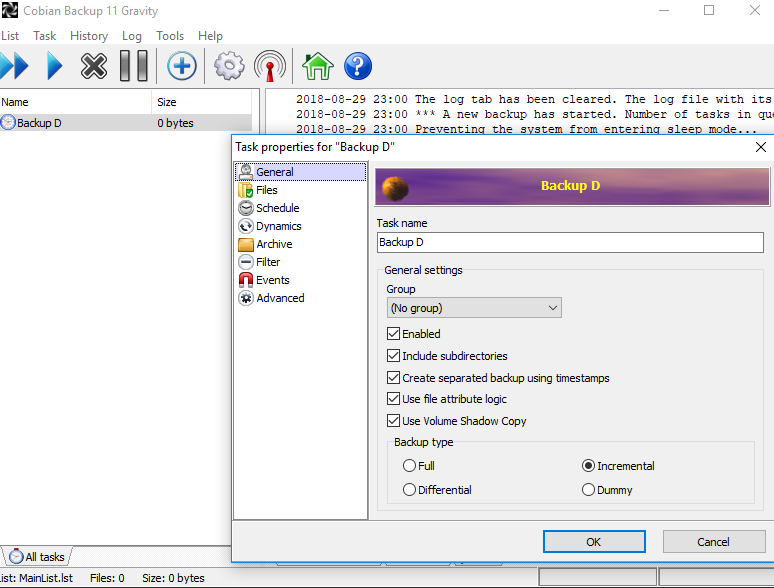
\includegraphics[width=8cm]{chapters/10-storage/img/cobian-img.png}
	\caption{Aplicația pentru replicarea datelor pe Windows: Cobian Backup}
	\label{fig:storage-cobian}
\end{figure}

\section{Anexă: Montarea dispozitivelor}
\label{sec:storage-mount}

Pentru a putea folosi un dispozitiv de stocare într-un sistem de calcul, acesta
trebuie montat. În cazul sistemelor Windows, dispozitivele sunt montate automat.
În cazul sistemelor Linux, acestea nu sunt întotdeauna montate (mai ales dacă
sistemul nu dispune de un GUI). Cazul cel mai des întâlnit este dat de montarea
unui stick USB. La inserarea unui stick USB într-o unitate de calcul, veți
observa în log-urile sistemului (rulați comanda \cmd{dmesg}), faptul ca acesta a
fost detectat, precum și litera alocată acestuia (în cazul de față observați că
este \file{/dev/sdb}):

\begin{screen}
usb 3-5: new high-speed USB device number 4 using xhci_hcd
usb 3-5: New USB device found, idVendor=abcd, idProduct=1234
usb 3-5: New USB device strings: Mfr=1, Product=2, SerialNumber=3
usb 3-5: Product: 1
usb 3-5: Manufacturer: 1
usb 3-5: SerialNumber: 60A44C3D7ECDAF710000058E
usb-storage 3-5:1.0: USB Mass Storage device detected
scsi host5: usb-storage 3-5:1.0
usbcore: registered new interface driver usb-storage
usbcore: registered new interface driver uas
scsi 5:0:0:0: Direct-Access     General  UDisk            5.00 PQ: 0 ANSI: 2
sd 5:0:0:0: Attached scsi generic sg2 type 0
sd 5:0:0:0: [sdb] 15728640 512-byte logical blocks: (8.05 GB/7.50 GiB)
sd 5:0:0:0: [sdb] Write Protect is off
sd 5:0:0:0: [sdb] Mode Sense: 0b 00 00 08
sd 5:0:0:0: [sdb] No Caching mode page found
sd 5:0:0:0: [sdb] Assuming drive cache: write through
 sdb:
sd 5:0:0:0: [sdb] Attached SCSI removable disk
\end{screen}

Dacă dorim să îl folosim, acesta trebuie montat:

\begin{screen}
root@monitor ~]#  mount /dev/sdb /mnt/part/
root@monitor ~]#  mount | grep sdb
/dev/sdb on /mnt/part type vfat (rw,relatime,fmask=0022,dmask=0022,codepage=437,iocharset=iso8859-1,shortname=mixed,errors=remount-ro)
\end{screen}

Se poate observa că am montat cu succes stick-ul USB reprezentat în sistemul de
operare Linux prin \file{/dev/sdb} în calea \file{/mnt/part}. Am verificat dacă
a fost montat folosind comanda mount. Se observă că acesta a fost formatat
folosind sistemul de fișiere VFAT.

Deseori companiile care produc software ne pun la dispoziție produsele sub forma
unui fișier cu extensia .iso predestinat scrierii pe un CD/DVD. Pentru a accesa
conținutul acestuia fără a-l scrie pe un suport fizic, putem folosi comanda
\cmd{mount} și parametrul \texttt{-o mount} prin care specificăm faptul că nu
vom monta un disc fizic:

\begin{screen}
[root@monitor ~]# mount -o loop test.iso /mnt/
[root@monitor ~]# ls -l /mnt/
total 108
-rw-rw-r-- 1 root root    14 May  2 14:28 CentOS_BuildTag
drwxr-xr-x 3 root root  2048 May  3 23:34 EFI
-rw-rw-r-- 1 root root   227 Aug 30  2017 EULA
-rw-rw-r-- 1 root root 18009 Dec 10  2015 GPL
drwxr-xr-x 3 root root  2048 May  3 23:45 images
drwxr-xr-x 2 root root  2048 May  3 23:34 isolinux
drwxr-xr-x 2 root root  2048 May  3 23:34 LiveOS
drwxrwxr-x 2 root root 71680 May  4 00:03 Packages
drwxrwxr-x 2 root root  4096 May  4 00:06 repodata
-rw-rw-r-- 1 root root  1690 Dec 10  2015 RPM-GPG-KEY-CentOS-7
-rw-rw-r-- 1 root root  1690 Dec 10  2015 RPM-GPG-KEY-CentOS-Testing-7
-r--r--r-- 1 root root  2883 May  4 00:07 TRANS.TBL
\end{screen}

O altă aplicație a noțiunii de montare o reprezintă accesibilitatea datelor
peste rețea din sistemul nostru de fișiere. Dacă dispunem de un server la
distanță, ce are serviciul de SSH funcțional, putem monta sistemul acestuia de
fișiere folosind utilitarul sshfs. Primul pas este instalarea acestuia:

\begin{screen}
[root@monitor ~]# apt-get install sshfs
\end{screen}

Acum vom monta un sistem de fișiere la distanță:

\begin{screen}
[root@monitor ~]# sshfs root@hp-wn01:/root/ /mnt/
[root@monitor ~]# mount | grep mnt
root@hp-wn01:/root/ on /mnt type fuse.sshfs (rw,nosuid,nodev)
[root@monitor ~]# ls -l /mnt/
total 4304336
-rw------- 1 root root       1285 Nov 13  2015 anaconda-ks.cfg
\end{screen}

După cum se poate observa, conținutul directorului /root de pe mașina cu numele
hp-wn01 a fost montat local. Partiția se poate demonta folosind comanda umount:

\begin{screen}
[root@monitor ~]# umount /mnt/
[root@monitor ~]# mount | grep mnt
[root@monitor ~]#
\end{screen}


Un alt caz particular al mecanismului de montare pe Linux îl reprezintă montarea
partițiilor de Windows cu sistem de fișiere NTFS. Pentru acest lucru trebuie să
instalați pachetul \textit{ntfs-3g}:
\begin{screen}
[root@monitor ~]# apt-get install ntfs-3g
\end{screen}

Folosind comanda mount și parametrul \texttt{-t} care specifică tipul sistemului
de operare, puteți monta un sistem de fișiere NTFS:

\begin{screen}
[root@monitor ~]# mount -t ntfs /dev/sdb1 /mnt
\end{screen}

\subsection{Crearea unui disc ce are ca suport un fișier}
\label{sec:storage-mount-create}

În acest studiu de caz ne propunem să creăm un fișier de dimensiune 4GB pe care
să îl partiționăm, formatăm și montăm întocmai unui disc fizic.

Pentru a crea un fișier folosim comanda \cmd{dd}. Comanda \cmd{dd} este capabilă
să citească și să scrie pe/de pe orice dispozitiv fizic sau fișier, având doi
parametri centrali: \texttt{if=} pentru fluxul de intrare și \texttt{of=} pentru
fluxul de ieșire. Alți parametri care pot fi specificați pentru a control
fluxul de date sunt:

\begin{itemize}
	\item bs - block size; dimensiunea unui block de date
	\item count - câte blocuri va scrie
\end{itemize}

Pentru a genera un fișier de 4GB, vom alege dimensiunea blocului, 4MB, iar count
va fi 1KB. În total se vor transera 4GB (4MB * 1KB). Sursa de intrare a datelor
va fi dispozitivul virtual \file{/dev/zero} care generează zerouri:

\begin{screen}
[root@monitor ~]# dd if=/dev/zero of=usodisk bs=4M count=1K
1024+0 records in
1024+0 records out
4294967296 bytes (4.3 GB) copied, 53.9797 s, 79.6 MB/s
\end{screen}

Vom asocia fișierul creat anterior cu un dispozitiv de tip block folosind
modului de kernel loop și utilitarul \cmd{losetup}:

\begin{screen}
[root@monitor ~]# losetup /dev/loop0 usodisk
[root@monitor ~]# losetup -a
/dev/loop0: [0803]:3426957 (/root/usodisk)
\end{screen}

Vom partiționa fișierul întocmai unui disc folosind \cmd{fdisk}:

\begin{screen}
[root@monitor ~]# fdisk /dev/loop0
Device contains neither a valid DOS partition table, nor Sun, SGI or OSF disklabel
Building a new DOS disklabel with disk identifier 0x55de94a4.
Changes will remain in memory only, until you decide to write them.
After that, of course, the previous content won't be recoverable.


Warning: invalid flag 0x0000 of partition table 4 will be corrected by w(rite)


WARNING: DOS-compatible mode is deprecated. It's strongly recommended to
         switch off the mode (command 'c') and change display units to
         sectors (command 'u').


Command (m for help): p


Disk /dev/loop0: 4294 MB, 4294967296 bytes
255 heads, 63 sectors/track, 522 cylinders
Units = cylinders of 16065 * 512 = 8225280 bytes
Sector size (logical/physical): 512 bytes / 512 bytes
I/O size (minimum/optimal): 512 bytes / 512 bytes
Disk identifier: 0x55de94a4


      Device Boot      Start         End      Blocks   Id  System


Command (m for help): n
Command action
   e   extended
   p   primary partition (1-4)
p
Partition number (1-4): 1
First cylinder (1-522, default 1):
Using default value 1
Last cylinder, +cylinders or +size{K,M,G} (1-522, default 522):
Using default value 522


Command (m for help): p


Disk /dev/loop0: 4294 MB, 4294967296 bytes
255 heads, 63 sectors/track, 522 cylinders
Units = cylinders of 16065 * 512 = 8225280 bytes
Sector size (logical/physical): 512 bytes / 512 bytes
I/O size (minimum/optimal): 512 bytes / 512 bytes
Disk identifier: 0x55de94a4


      Device Boot      Start         End      Blocks   Id  System
/dev/loop0p1               1         522     4192933+  83  Linux
\end{screen}

Pentru a face disponibile partițiile, vom folosi utilitarul \cmd{kpartx}:

\begin{screen}
[root@monitor ~]# kpartx -a /dev/loop0
[root@monitor ~]# ls -l /dev/mapper/loop0p1
lrwxrwxrwx 1 root root 7 Aug 30 10:46 /dev/mapper/loop0p1 -> ../dm-0
\end{screen}

În acest moment putem formata partiția 1 și o putem monta:

\begin{screen}
[root@monitor ~]# mkfs.ext4 /dev/mapper/loop0p1
mke2fs 1.43-WIP (20-Jun-2013)
Discarding device blocks: done
Filesystem label=
OS type: Linux
Block size=4096 (log=2)
Fragment size=4096 (log=2)
Stride=0 blocks, Stripe width=0 blocks
262144 inodes, 1048233 blocks
52411 blocks (5.00%) reserved for the super user
First data block=0
Maximum filesystem blocks=1073741824
32 block groups
32768 blocks per group, 32768 fragments per group
8192 inodes per group
Superblock backups stored on blocks:
        32768, 98304, 163840, 229376, 294912, 819200, 884736


Allocating group tables: done
Writing inode tables: done
Creating journal (16384 blocks): done
Writing superblocks and filesystem accounting information: done


[root@monitor ~]# mount /dev/mapper/loop0p1 /mnt/
[root@monitor ~]# mount | grep mnt
/dev/mapper/loop0p1 on /mnt type ext4 (rw)
\end{screen}

În continuare vom demonta partiția, vom șterge intrarea creată de utilitarul
\cmd{kpartx} și vom șterge dispozitivul virtual \file{/dev/loop0}. Acest lucru
trebuie făcut atunci când ați terminat operațiile asupra discului reprezentat de
fișierul \file{usodisk}:

\begin{screen}
[root@monitor ~]# umount /mnt/
[root@monitor ~]# kpartx -d /dev/loop0
[root@monitor ~]# losetup -d /dev/loop0
\end{screen}

\section{Anexă: Logical Volume Manager}
\label{sec:storage-lvm}

Procesul de partiționare se poate aplica doar asupra unui disc fizic. Dacă în
sistem sunt montate două discuri, pentru fiecare din acestea trebuie realizată
partiționarea. În sisteme de tip Linux, pentru a rezolva acest neajuns, a fost
introdus conceptul de LVM \abbrev{LVM}{Logical Volume Manager} - Logical Volume
Manager. În cadrul acestuia există următoarele obiecte:

\begin{itemize}
	\item Physical Volume - sunt discurile fizice alte sistemului asociate LVM-ului
	\item Volume Group - format din unul sau mai multe discuri asociate anterior
	\item Logical Volume - alocate din spațiul disponibil într-unul din
		Volume Group-urile create anterior. Doar acesta este vizibil în
		sistemul de operare și poate fi formatat cu un sistem de
		fișiere.
\end{itemize}

Atunci când instalați o distribuție de Linux, aveți opțiunea de a activa LVM-ul.
Utilitatea acestuia apare atunci când mai adăugați un disc și doriți să măriți
dimensiunea partițiilor existente.

În exemplul următor vom investiga configurația unui sistem de are activat LVM-ul:

\begin{itemize}
	\item Vom lista discurile fizice:

\begin{screen}
mamba:~# pvs
  PV         VG      Fmt  Attr PSize PFree
  /dev/md2   storage lvm2 a-   1.14t 130.47g
\end{screen}

	\item Se observă un disc denumit /dev/md2 cu capacitatea 1.14TB. Vom
		lista acum volumele:

\begin{screen}
mamba:~# vgs
  VG      #PV #LV #SN Attr   VSize VFree
  storage   1   6   0 wz--n- 1.14t 130.47g
\end{screen}

	\item Se observă un singur volum denumit \textit{storage}. Observați din
		ce discuri fizice este compus:

\begin{screen}
mamba:~# pvdisplay /dev/md2
  --- Physical volume ---
  PV Name               /dev/md2
  VG Name               storage
  PV Size               1.14 TiB / not usable 4.00 MiB
  Allocatable           yes
  PE Size               4.00 MiB
  Total PE              299641
  Free PE               33401
  Allocated PE          266240
  PV UUID               M9WAFG-pf9x-Uo0j-7r8N-spOy-5evy-tt0cyc
\end{screen}

	\item Vom lista acum volumele logice, cele care sunt vizibile sistemului
		de operare:

\begin{screen}
mamba:~# lvs
  LV       VG      Attr   LSize   Origin Snap%  Move Log Copy%  Convert
  home     storage -wi-ao  20.00g
  labs     storage -wi-ao 200.00g
  projects storage -wi-ao 200.00g
  rosedu   storage -wi-ao 100.00g
  swarm    storage -wi-ao 500.00g
  titan    storage -wi-ao  20.00g
\end{screen}


	\item Observați că toate acestea sunt prezente în calea /dev:

\begin{screen}
mamba:~# ls -l /dev/mapper/storage-*
lrwxrwxrwx 1 root root 7 Aug  9 07:18 /dev/mapper/storage-home -> ../dm-0
lrwxrwxrwx 1 root root 7 Aug  9 07:18 /dev/mapper/storage-labs -> ../dm-2
lrwxrwxrwx 1 root root 7 Aug  9 07:18 /dev/mapper/storage-projects -> ../dm-3
lrwxrwxrwx 1 root root 7 Aug  9 07:18 /dev/mapper/storage-rosedu -> ../dm-1
lrwxrwxrwx 1 root root 7 Aug  9 07:18 /dev/mapper/storage-swarm -> ../dm-5
lrwxrwxrwx 1 root root 7 Aug  9 07:18 /dev/mapper/storage-titan -> ../dm-4
\end{screen}

\end{itemize}

În \labelindexref{Figura}{fig:lvm-struct} este reprezentat grafic incluziunea
dintre Physical Volume, Volume Group și Logical Volume.

\begin{figure}[htbp]
	\centering
	\def\svgwidth{\columnwidth}
	\includesvg{chapters/10-storage/img/lvm-struct.svg}
	\caption{Componentele LVM}
	\label{fig:lvm-struct}
\end{figure}

\section{Anexă: Replicarea datelor}
\label{sec:storage-replicare}

În general, datele salvate pe sistemele de stocare sunt critice. Defectarea
sistemelor de stocare este iminentă mai ales din cauza faptului că HDD-urile
sunt sensibile la șocuri, iar SSD-urile au un număr limitat de scrieri din
proiectare. Pentru a preveni pierderea iremediabilă a datelor, datele sunt
replicate prin diverse mecanisme pe mai multe unități de stocare.

Replicarea datelor pe discuri diferite se poate realiza automat la nivel de bloc
de date atunci când acestea sunt trimise de către sistemul de operare.
Mecanismul prin care se face este lucru se numește RAID \abbrev{RAID}{Redundant
Array of Independent/Inexpensive Disks} (Redundant Array of
Independent/Inexpensive Disks). Protocolul RAID poate fi implementat în hardware
de către controller-ul de stocare sau în software de către sistemul de operare.
RAID-ul din hardware dispune de un protocol proprietar, cu metadate diferite de
la vendor la vendor. Așadar un volum (set de discuri) configurate în RAID nu
poate fi mutat pe un alt sistem.

RAID-ul dispune de mai multe niveluri de protecție:

\begin{itemize}
	\item RAID0 - datele sunt distribuite pe toate discurile configurate. Nu
		există nici un nivel de replicare (ex. Dacă avem două discuri
		configurate în RAID0 va rezulta un volum ce are capacitatea
		celor două discuri însumată, fără nici un nivel de replicare)
	\item RAID1 - datele sunt scrise pe 2 din discurile configurate. Dacă un
		disc se va defecta, celălalt va deține informația (ex. Dacă avem
		două discuri configurate în RAID1 va rezulta un volum ce are
		capacitatea celui mai mic dintre discuri, cu un nivel de
		replicare a datelor)
	\item RAID5 - datele sunt scrise pe 1 disc și se mai scrie o sumă de
		control pe un alt disc. Cu ajutorul sumelor de control, datele
		pot fi recuperate dacă un disc pică. Necesită cel puțin 3
		discuri. Poate pica un singur disc, iar datele rămân
		disponibile.
	\item RAID10 - combinația dintre RAID0 si RAID1 (datele sunt distribuite
		și replicate). Acesta asigură unul dintre cele mai bune niveluri
		de protecție și performanță crescută
\end{itemize}

În \labelindexref{Figura}{fig:raid-types} sunt reprezentate grafic modurile de
funcționare RAID prezentate mai sus. Pe lângă acestea mai există și RAID6, care
este asemănător RAID5, dar are două discuri pe care se reține paritatea. Așadar
pot pica 2 discuri la un moment dat, iar datele sunt disponibile în continuare.

\begin{figure}[htbp]
	\centering
	\def\svgwidth{\columnwidth}
	\includesvg{chapters/10-storage/img/raid-types.svg}
	\caption{Niveluri RAID}
	\label{fig:raid-types}
\end{figure}

În sistemele bazate pe Linux, RAID-ul software este implementat prin modulul MD
(Multiple Device). Cu ajutorul acestuia se pot configura două sau mai multe
discuri fizice să participe în formarea unei grupări RAID:

\begin{screen}
mamba:~# cat /proc/mdstat
Personalities : [raid1] [raid6] [raid5] [raid4]
md2 : active raid5 sda3[0] sdc3[2] sdb3[1]
      1227333632 blocks level 5, 64k chunk, algorithm 2 [3/3] [UUU]
\end{screen}


Se observă dispozitivul \textit{md2}, configurat în mod RAID5, folosind
partițiile sda3 sdc3 și sdb3, toate fiind disponibile.

Replicarea folosind mecanismul RAID este utilă atunci când sistemul rulează și
dorim protecție permanentă a datelor. Acest lucru este costisitor: pierdem
spațiu util și performanța este mai scăzută. Mecanismul RAID se folosește cu
precădere în sistemele de tip server. Pentru sistemele desktop/laptop se
folosesc alte mecanisme cum ar fi:

\begin{itemize}
	\item Crearea unei imagini a întregului disc
	\item Snapshot folosind sistemul de fișiere
	\item Copierea fișierelor pe un disc extern sau pe un alt dispozitiv
		peste rețea
\end{itemize}

Crearea unei imagini a întregului disc este utilă atunci când dorim să refacem
un sistem rapid ce a fost afectat de un defect hardware sau de un virus (e.g.,
crypto-locker - tot discul a fost criptat). Un alt caz în care este util să
folosim imaginea unui disc este atunci când dorim replicarea aceleiași
configurații pe mai multe sisteme identice. Un program ce vă poate ajuta să
faceți acest lucru atât pe Linux, cât și pe Windows este: Clonezilla
(https://clonezilla.org/).

Snapshot folosind sistemul de fișiere se poate face doar dacă acesta suportă.
Cel mai cunoscut sistem de fișiere cu această facilitate este ZFS
(https://www.freebsd.org/doc/handbook/zfs.html), disponibil în general pe
sistemele server.

Copierea fișierelor pe un disc extern sau pe un alt dispozitiv peste rețea este
o altă modalitate de replicare a datelor. Această metodă este utilă atunci când
dorim salvarea unui director din tot sistemul de fișiere sau atunci când dorim
să facem replicare incrementală. Replicarea incrementală va transfera doar
diferențele între fișiere, iar în acest mod se poate realiza și o versionare a
acestora (se pot reține mai multe versiuni ale aceluiași fișier). Cel mai
cunoscut utilitar pentru Linux în rezolvarea acestui lucru este \cmd{rsync}. Un
exemplu pentru Windows gratuit îl constituie: \cmd{Cobian}.

Copierea datelor se poate realiza pe un disc extern conectat pe USB sau pe un
alt dispozitiv în rețea. În general în rețea avem alte servere pe care copiem
datele sau avem dispozitive speciale de stocare denumite NAS
\abbrev{NAS}{Network Attached Storage} (Network Attached
Storage). Un NAS este un sistem de calcul cu un software specializat pentru
accesarea și stocarea datelor. Acesta expune în rețea o multitudine de
protocoale de acces (http, ftp, nfs, cifs) compatibile cu aproape toate
sistemele de operare.
